\documentclass[%
 aip,
% jmp,
% bmf,
% sd,
% rsi,
cp,  % Conference Proceedings
 amsmath,amssymb,%nobibnotes,
% preprint,%
 reprint,%
%author-year,%
%author-numerical,%
]{revtex4-2}

\usepackage{graphicx}% Include figure files
\usepackage{dcolumn}% Align table columns on decimal point
\usepackage{bm}% bold math
%\usepackage[mathlines]{lineno}% Enable numbering of text and display math
%\linenumbers\relax % Commence numbering lines

\usepackage[utf8]{inputenc}
\usepackage[T1]{fontenc}
%% Loads a Times-like font. You can also load
%% {newtxtext,newtxtmath}, but not {times},
%% {txfonts} nor {mathtpm} as these packages
%% are obsolete and have been known to cause problems.
\usepackage{mathptmx}

\begin{document}

\title{Monte Carlo study of the systematic errors in the measurement of the ${}^{15}$N ions scattering from ${}^{10,11}$B}% Force line breaks with \\

\author{Ilyas Satyshev} % Write as First name Surname
 \email[Corresponding author: ]{satyshev@jinr.ru}
 \affiliation{
 Joint Institute for Nuclear Research,
 6 Joliot-Curie street, Dubna, Moscow Region, Russia, 141980% Force line breaks with \\ if necessary
}
\affiliation{%
 The Institute of Nuclear Physics, 1 Ibragimova street, Almaty, the Republic of Kazakhstan, 050032
% Force line breaks with \\ if necessary
}%

\author{ Sergey G. Belogurov}%
 \affiliation{
 Joint Institute for Nuclear Research,
 6 Joliot-Curie street, Dubna, Moscow Region, Russia, 141980% Force line breaks with \\ if necessary
}

\author{ Mikhail Y. Kozlov}%
 \affiliation{
 Joint Institute for Nuclear Research,
 6 Joliot-Curie street, Dubna, Moscow Region, Russia, 141980% Force line breaks with \\ if necessary
}
\affiliation{
 Bauman Moscow State Technical University, 5 Baumanskaya-2 street, Moscow, Russia, 105005% Force line breaks with \\ if necessary
}
\author{ Bakytbek Mauyey}
 \affiliation{
 Joint Institute for Nuclear Research,
 6 Joliot-Curie street, Dubna, Moscow Region, Russia, 141980% Force line breaks with \\ if necessary
}
\affiliation{%
 The Institute of Nuclear Physics, 1 Ibragimova street, Almaty, the Republic of Kazakhstan, 050032
% Force line breaks with \\ if necessary
}%

\author{ Egor V. Ovcharenko }
 \affiliation{
 Joint Institute for Nuclear Research,
 6 Joliot-Curie street, Dubna, Moscow Region, Russia, 141980% Force line breaks with \\ if necessary
}
\affiliation{%
 Justus-Liebig-Universität, Ludwigstraße 23, Gießen, Germany, 35390
% Force line breaks with \\ if necessary
}%

\author{ Vitaly N. Schetinin }
 \affiliation{
 Joint Institute for Nuclear Research,
 6 Joliot-Curie street, Dubna, Moscow Region, Russia, 141980% Force line breaks with \\ if necessary
}

\date{\today} % It is always \today, today, but any date may be explicitly specified
              % Not printed for conference proceedings

\begin{abstract}
A series of experiments on the elastic scattering of ${}^{15}$N ions from ${}^{10,11}$B has been done at U-200P cyclotron at Heavy Ion Laboratory of the Warsaw University using the charged particles detection system ICARE. The measured relative differential cross sections are used for obtaining the theoretical interpretation in terms of the Optical Model for pure elastic scattering and Distorted wave Born Approximation for the cluster transfer mechanism. The accuracy of the interpretation depends on the systematic errors of the experiment. This work reports on a Monte Carlo (MC) study of such errors using the ExpertRoot simulation and analysis framework based on the FairRoot package. Influence of such factors as angular, spatial and energy spread of the beam, energy loss and multiple scattering in the target and the dimension of the detector slit on the angular resolution of the detector and the reconstructed relative differential cross section are investigated. The MC model allowed to study the influence of the ion identification and detection efficiency and the energy resolution as well. However, in the given experiment these factors were not of any importance. As a result, it has been demonstrated that the reconstructed differential cross section is slightly different from the input one.  The main reason for this distinction is the beam spot size at the target. Influence of the slit length is negligible; hence it can be increased for better detection efficiency. The developed software will be used for planning and analysing similar experiments in the future.
\end{abstract}

\maketitle

\section{Introduction}
Elastic scattering of ${}^{15}$N ions from ${}^{10,11}$B at low energy is a probe for the internal structure of ${}^{15}$N nucleus. A series of experiments at Elab(${}^{15}$N) = 43 MeV has been done at U-200P cyclotron at Heavy Ion Laboratory, of the Warsaw University [1]. Remarkable increase in differential cross section at large angles which cannot be explained by optical model has been observed. Such behavior of the cross section can be reproduced only taking into account the contribution of the $\alpha$-cluster transfer mechanism in the distorted waves Born approximation (DWBA) method. \\
The experiments have been performed using the charged particles detection system ICARE [2]. The detector system has very high detection and identification efficiencies and simple geometry that allows deriving the relative differential cross section from the count rate with a good accuracy using a simple formula:

\begin{eqnarray}
 \frac{ \frac{d\sigma}{d\Omega}(\theta) }{\sigma_{tot}} = \frac{N}{N_0 d\Omega_{det}},
\end{eqnarray}

where

\begin{eqnarray}
  \sigma_{tot} = 2\pi \int\limits_{5^{0}}^{180^{0}} sin(\theta)\frac{d\sigma}{d\Omega}(\theta)d\theta,
 \end{eqnarray}
and N$_{0}$ is a full projectiles number interacted with the target.

Nevertheless, the beam emittance, finite thickness of the target and the size of the detector slit lead to certain systematic deviation of the measured relative cross section w.r.t its true value. In this work, such deviations were investigated using Monte Carlo (MC) simulation within the ExpertRoot (ER) [3].

ER is a framework for simulation of detector`s response, event reconstruction and real data analysis in low energy nuclear physics with radioactive beams. ExpertRoot is used for the EXPERT [4] project at SuperFRS (FAIR) and for the experiments at ACCULINNA-2 fragment-separator a [5].  ER inherits its approaches and methodology for developing software for entire life cycle of an experiment from FAIRRoot[6]. It adds the functionality needed for specific experiments and setups, It uses Root[7] for data storage and analysis and Geant4 [8] as a simulation engine.

The obtained results can be used for improving the theoretical interpretation of the experimental data. The developed method takes into account realistic descriptions of the energy deposit processes in the detector itself and signal processing in the readout and data acquisition systems. It is intended to be used for other similar experiments.

\section{The experiment and its Monte Carlo simulation}

The experimental setup (Fig. 1) consists of: a collimator for the 15N beam, ${}^{11}$B target and four identical detectors. Each detector is a combination of a gas ionization chamber and a silicon sensor, it allows identification of ions by the dE vs. E method. The aperture of the detector is defined by a vertical slit 2x4 mm in the aluminum cap. In order to measure angular dependence of the counting rate the detectors were moved with step of $1^0$  from $5^0$ to 4$5^0$ in Lab. Note that the angle of 4$5^0$ in the lab corresponds to $\theta$-angle of 9$0^0$  in Center of mass (CM) reference frame. Both ${}^{15}$N and ${}^{10,11}$B ions can be identified and counted by the detector. CM $\theta$-angle less than 9$0^0$  are accessible when ${}^{15}$N ions are detected while detection of ${}^{10,11}$B ions allow to explore the CM $\theta$-angle bigger than 9$0^0$.

\begin{figure}[h!]
\begin{minipage}[h]{0.50\linewidth}
\center{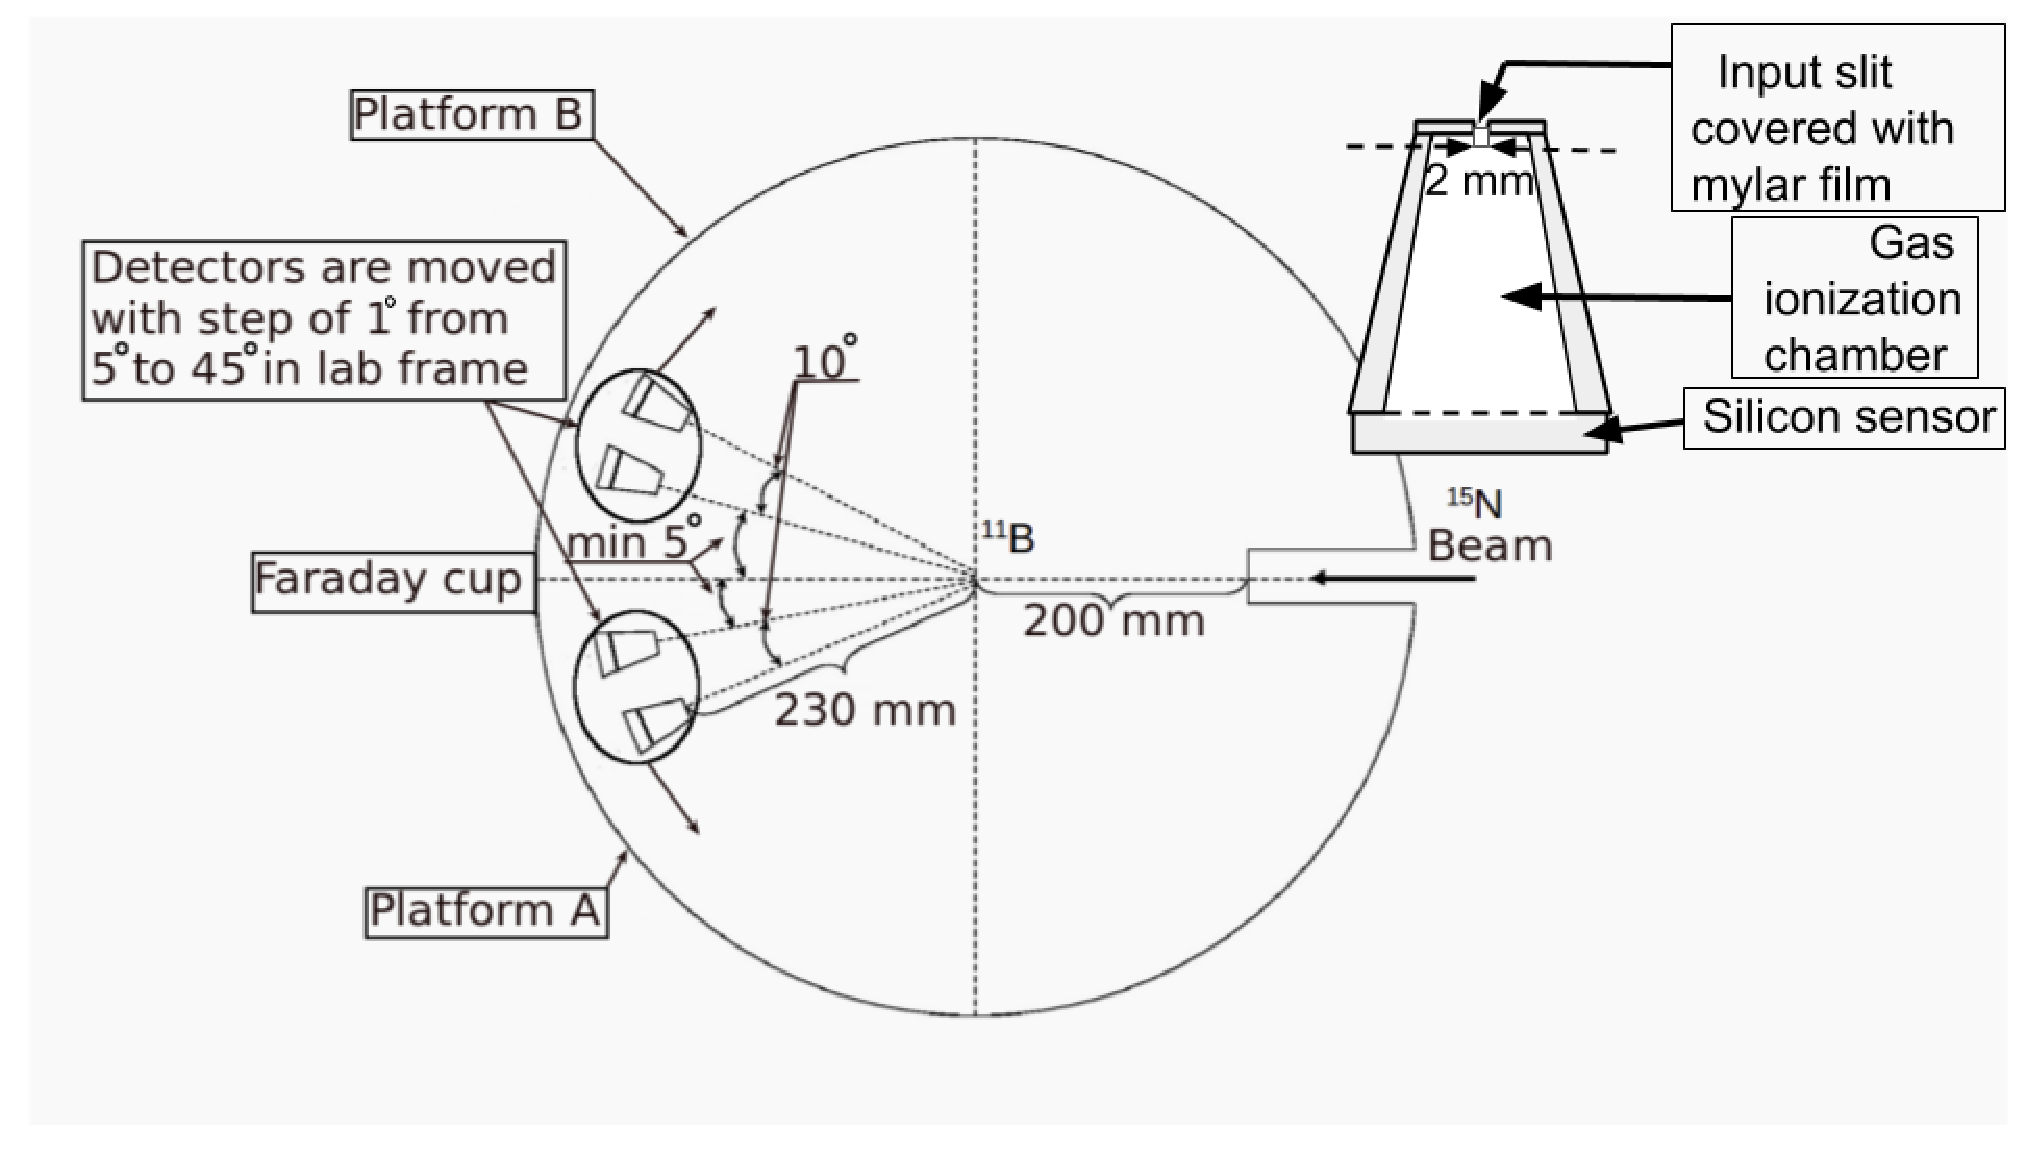
\includegraphics[width=1\linewidth]{fig_1.eps} \\ (a)}
\end{minipage}
\hfill
\begin{minipage}[h]{0.38\linewidth}
\center{\includegraphics[width=1\linewidth]{fig_2.eps} \\ (b)}
\end{minipage}
\vspace{0.05cm}
\caption{(a) Scheme of the Experimental set up. (b) Scheme of used detector. }
\label{ris:fig1}
\end{figure}

The following features of ER are used in this work:
\begin{enumerate}
\item The interaction point inside the target is defined according to the user-defined distribution. The incident ion is transported till the interaction point taking into account ionization losses and multiple scattering.
\item The velocity of the incident ion in the interaction point is used for defining the CM reference frame.
\item A user-defined interaction is called. The incident ion is killed and the interaction products are put into the particle stack. For the case of the elastic scattering the user has to provide only the angular distribution in the CM reference frame in the form of the tabulated cumulative distribution function (CDF).
\item The user can select the ranges of the CM $\theta$ and $\phi$-angles to be sampled in order to hit with the scattered ions only the slit of the detector and some zone around it thus saving the simulation time.  Corresponding re-normalization of the total number of the events is automatically performed.
\end{enumerate}

\section{Results and discussion}

The MC study included two stages. At the first stage the deterioration of the angular resolution due to different physical and geometrical factors  was investigated, at the second one we studied how the detection system distorts the derived differential cross section curves w.r.t. the input ones.

\begin{figure}[h]
\center{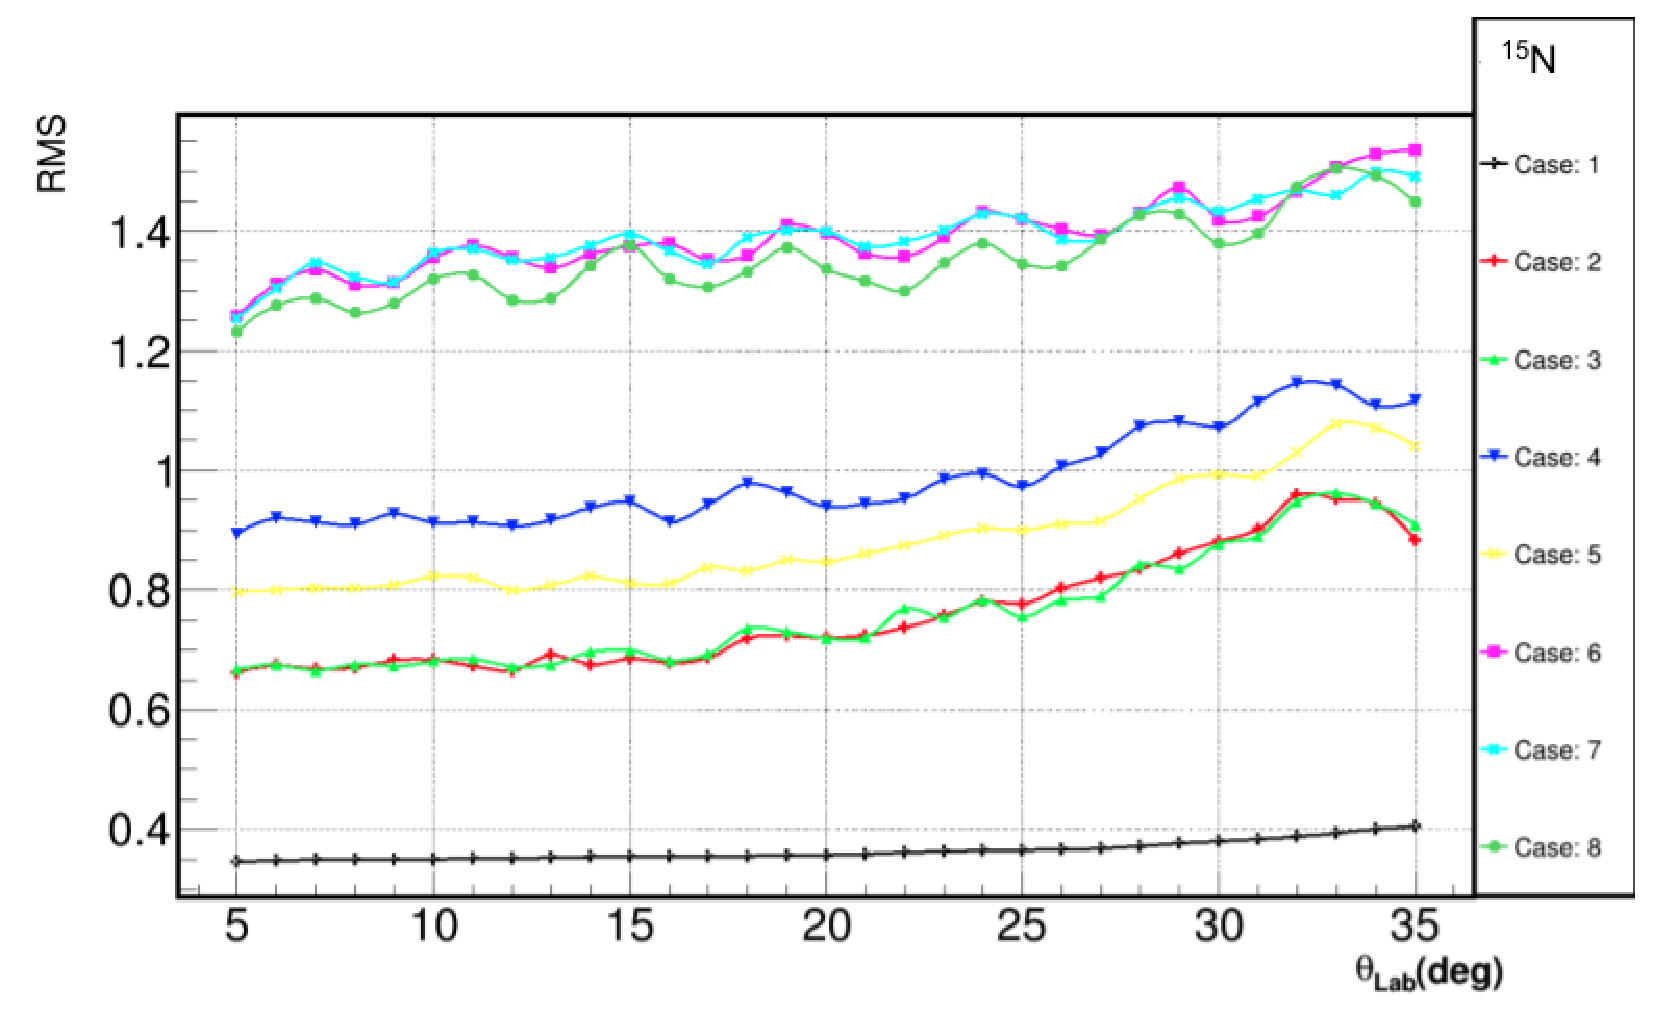
\includegraphics[width=1\linewidth]{fig_3.eps}}
\caption{The angular resolution rms [deg] vs. Lab $\theta$-angle curves for different cases.}
\label{ris:fig3}
\end{figure}

\begin{figure}[h]
\center{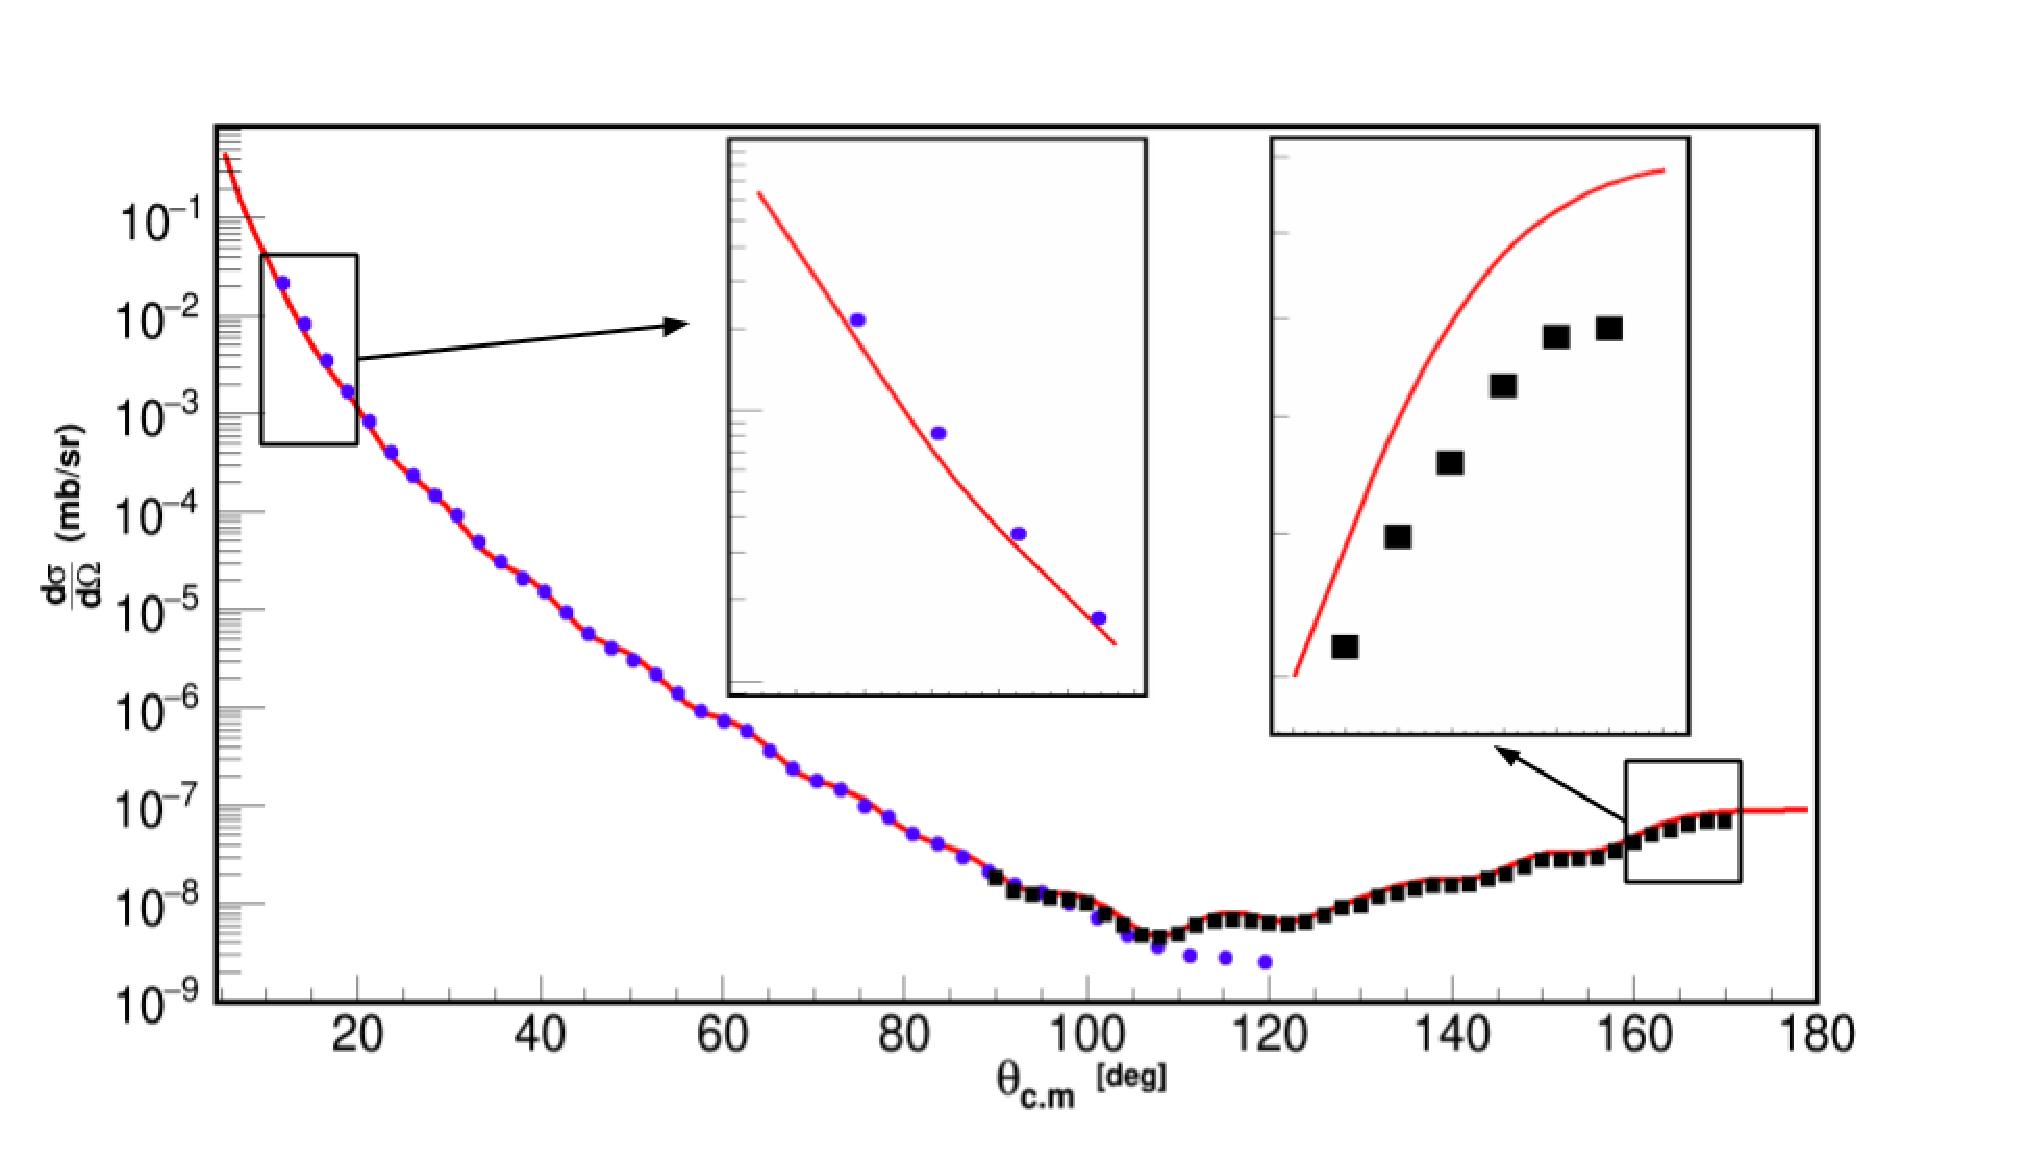
\includegraphics[width=1\linewidth]{fig_4.eps}}
\caption{It is shown measured cross section as a function of the scattering angle in the CM.}
\label{ris:fig4}
\end{figure}

The angular resolution was defined as rms deviation of CM $\theta-$angle detected for Lab $\theta$-angle detectors position.
In the Fig. 2 the angular resolution vs. Lab $\theta$-angle curves are shown for different cases. We started from the ideal case with the beam along the Z-axis, without the target but with the realistic slit of the detector (Case 1) and introduced step by step the following realistic features: the 7-micron-thick ${}^{11}$B target (Case 2), energy spread of the ${}^{15}$N ion beam (42-43 MeV, uniform) (Case 3), spread of the $\theta$-angle of the ${}^{15}$N ion beam ($\sigma$ = 5 mrad) (Case 4),  spread of the $\phi$-angle of the ${}^{15}$N ion beam (0-2$\pi$, uniform) (Case 5), the X spread of the beam spot on the target (-0.5-0.5 cm, uniform) (Case 6), the Y spread of the beam spot on the target (-0.5-0.5 cm, uniform) (Case 7), the beam collimator (hole diameter is 1.5 cm)  (Case 8).


In the Fig. 2 one can see that the angular resolution deteriorates by the factor almost 4 when all the discussed non idealities are taken into account. The statistical error of each point does not exceed $\pm$1$\%$. Wave-like behavior is statistically significant, but its cause is not clear. The main factors deteriorate angular resolutions are ${}^{11}$B target thick and X spread of the $\theta$-angle of the ${}^{15}$N ion beam.

The Fig. 2 shows how the detection system distorts the input differential cross section curves. Unlike the real experiment, where normalization is used, in the MC study we have enough data for deriving the absolute cross section. Here the red line corresponds to the input cross-section and the blue and black points correspond to the restored one. There are three main effects. First is that the reconstructed cross section is slightly smaller than the input one. It is because some scattered ions go above and below the detector slit. This effect is not relevant for the experiment where the relative cross section is measured. The second is that the measured dependence becomes less steep at the small angles than the original curve. The third is that the wave-like structure of the original curve becomes less prominent. The last two effects are relevant for the experiment and are due to the non-ideal angular resolution of the entire set up.

\section{Conclusion}

MC simulations of the experiment on the elastic scattering of 15N from 11B have been done. Systematic influence of some physical and geometrical factors on the results has been studied. It has been demonstrated that the reconstructed differential cross section is slightly different from the input one. The main reason for this distinction is the beam spot size at the target. Influence of the detector slit height is negligible; hence it can be increased for better detection efficiency The developed software will be used for planning and analysis of similar experiments in the future.

\section{References}

\begin{enumerate}
\item N. Burtebayev et al., Acta Physica Polonica B Proceedings Supplement, Vol. 11 (2018) No 1, pp. 99–107.
\item E. Piasecki, M. Antczak, J. Devine (2007). Project ICARE at HIL. Annual report 2006. Warsaw University. Heavy       Ion Laboratory, page 38.
\item ExpertRoot core team, ExpertRoot, Website, available online at https://e.ru; last visited on June 12th 2019.
\item H. Geissel, O. Kiselev, I. Mukha, et al., "Expert (exotic Particle Emission and Radioactivity by Tracking) Studies at the Super-FRS Spectrometer", 2015, Exotic Nuclei: EXON-2014 - Proceedings of International Symposium.
\item A.S. Fomichev, L.V. Grigorenko, S.A. Krupko, S.V. Stepantsov and G.M. Ter-Akopian "The ACCULINNA-2 project: The physics case and technical challenges", Eur. Phys. J. A (2018) 54: 97
\item FairRoot core team, FairRoot, Website, available online at http://fairroot.gsi.de; last visited on June 20th 2019.
\item The Root Team, ROOT Homepage, Website, available online at https://root.cern.ch/; last visited on July 1 2019.
\item S. Agostinelli et al., Nucl. Instrum. Meth. A 506 (2003) 250-303

\end{enumerate}

\end{document}
%
% ****** End of file aipsamp.tex ******
